\lesson{6}{Mar 04 2022 Fri (21:13:37)}{Solve quadratic inequality}{Unit 4}

Let's say we have $x^{2} -x \ge 12$. When dealing with an equation where $x =
a$, $x$ has a set value. But if you're dealing with an inequality, $x$ has a
range of values.

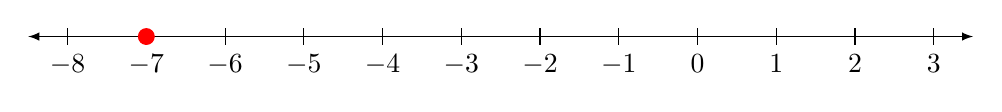
\begin{tikzpicture}
  \draw[latex-latex] (-8.5,0) -- (3.5,0);
  \foreach \x in {-8,-7,-6,-5,-4,-3,-2,-1,0,1,2,3}
  \draw[shift={(\x,0)},color=black] (0pt,3pt) -- (0pt,-3pt);
  \foreach \x in {-8,-7,-6,-5,-4,-3,-2,-1,0,1,2,3}
  \draw[shift={(\x,0)},color=black] (0pt,0pt) -- (0pt,-3pt) node[below] 
  {$\x$};

  \draw [red,fill=red,radius=0.1] (-7,0) circle;
\end{tikzpicture}

\newpage
